
\section{Experimental Results}\label{sec:exp}


Here you evaluate your work using experiments. You start again with a
very short summary of the section. The typical structure follows.

\mypar{Experimental setup} The experiments were executed on a Intel Xeon Phi 7120 coprocessor. It consists of 61 cores and 16 GB of GDDR5 memory with a theoretical bandwidth of 352 GB/sec.
For compilation the Intel Compiler version 15.0.0 20140723 was used with the following flags: -fopenmp -std=c++11 -mmic -Wall -qopt-report3 -qopt-report-phase=vec -O3 .

The benchmarks focus on the tokenizer and the matcher. To generate test data, we used the XML benchmark project XMark \todo{reference}. To measure the scalability of the tokenizer 100 test runs were conducted. For each run, a input file with the size of 2 GB was used which contained 61'113'640 tokens. First, we measured the performance of the tokenizer working with 1 thread. Then we increased the number of threads to 2, 4, 8, 16, 32, 60, 120, 180 and 240. Each experiment was run ten times. The results were built with the average of these runs. Similarly, the matcher was tested with files of the sizes 2 GB (27'620'104 tokens), 4 GB (55'236'244 tokens) and 8 GB (110'467'124 tokens). For each file 10 different experiment was run. The first experiment matched 1 query, i.e. running with 1 thread, the second matched 2 queries and the following experiments matched 4, 8, 16, 32, 60, 120, 180 and 240 queries. Again, each experiment was conducted 10 times and the result is the average of the runs.

\mypar{Results}
\begin{figure}\centering
  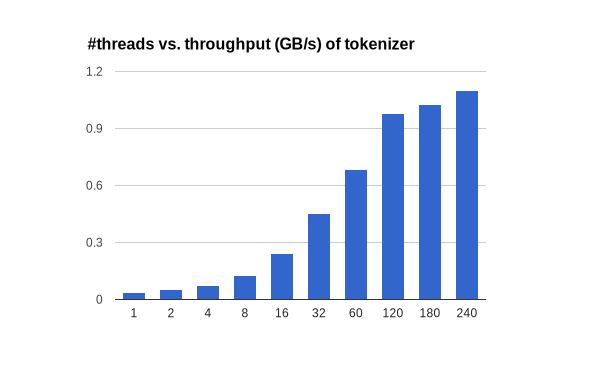
\includegraphics[scale=.66]{img/tokenizer_throughput.eps}
  \caption{Throughput of the tokenizer in GB/s measured with different numbers of threads.
  \label{tokenizer_throughput}}
\end{figure}
The experiments reveal clearly, that the throughput of the tokenizer increases with the number of threads and in Fig.~\ref{tokenizer_throughput} nearly linear scaling can be seen. While the benefits of more threads are significant up to 120 threads, i.e. two threads per core, less performance can be gained from 120 up to 240 threads.

\begin{figure}\centering
  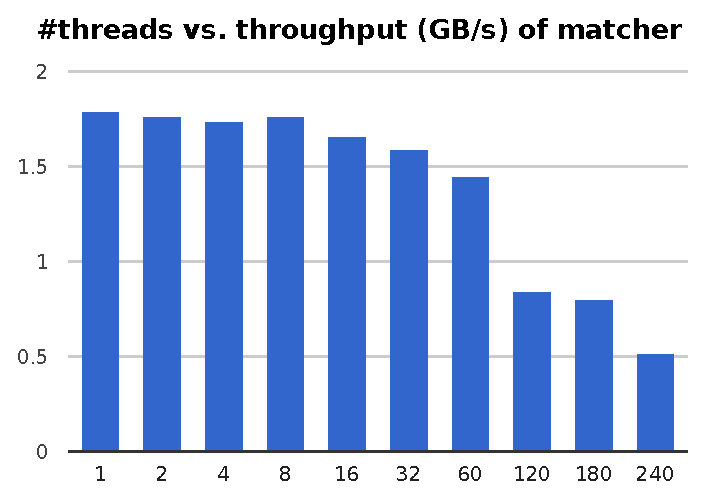
\includegraphics[scale=.66]{img/matcher_throughput.eps}
  \caption{Throughput in GB/s of the matcher with fixed input file size (2GB). Plotted against the number of threads.\label{matcher_throughput}}
\end{figure}
In Fig.~\ref{matcher_throughput} the throughput of the matcher against the numbers of queries, i.e. threads, is plotted. Up to 60 queries there is no significant drop of the performance, while after 120 queries the throughput plummets. Up to 60 threads weak scaling is observable. When the number of threads exceeds the number of cores the performance suffers.

Similarly in Fig.~\ref{matcher_performance} the increase of the processing time after 60 threads can be seen. While the different is not too drastic for files of 2 GB and 4 GB, a spike for 8 GB can be seen. We assume this is due to the memory access pattern of the Xeon Phi, which becomes apparent, when more threads operate at the same time on larger data. Pursuing experiments that confirm this assumption would exceed the format of this report.

\begin{figure}\centering
  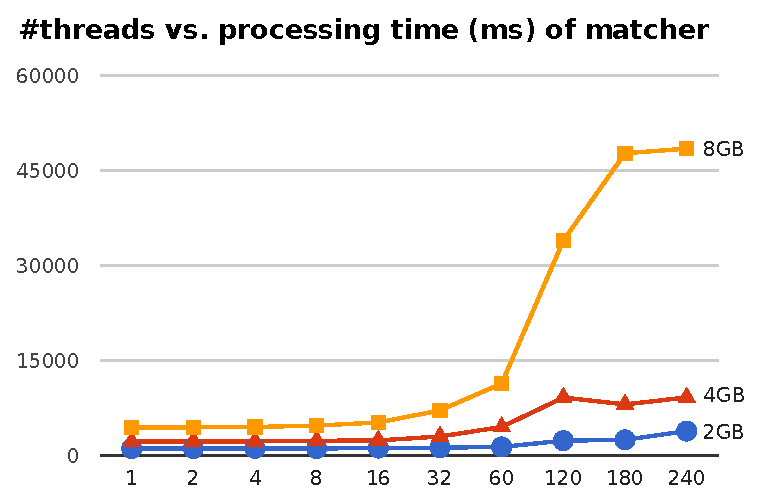
\includegraphics[scale=.66]{img/matcher_processing_time.eps}
  \caption{Processing time of the matcher for 2 GB, 4 GB and 8 GB XML files. Plotted against the number of queries, i.e. threads.\label{matcher_performance}}
\end{figure}